\documentclass[letterpaper,11pt]{article}
\usepackage{natbib}
\bibliographystyle{unsrtnat}
\usepackage{tabularx} % extra features for tabular environment
\usepackage{amsmath}
\usepackage{amsfonts}
\usepackage{mathtools}
\usepackage{graphicx} % takes care of graphic including machinery
\usepackage[margin=1in,letterpaper]{geometry} % decreases margins
%\usepackage{cite} % takes care of citations
\usepackage[final]{hyperref} % adds hyper links inside the generated pdf file
\graphicspath{ {./images/} }

\DeclarePairedDelimiter\floor{\lfloor}{\rfloor}  % improve math presentation
\hypersetup{
	colorlinks=true,       % false: boxed links; true: colored links
	linkcolor=blue,        % color of internal links
	citecolor=blue,        % color of links to bibliography
	filecolor=magenta,     % color of file links
	urlcolor=blue         
}
%+++++++++++++++++++++++++++++++++++++++

\begin{document}

\title{Discrete Math Question Set 3}
\author{Abrar Habib}
\date{October 26, 2022}
\maketitle


\begin{enumerate}
    \item [1.] Determine whether the relation R on the set of all integers is reflexive, symmetric, antisymmetric, and/or
    transitive, where $(x, y) \in R$ if and only if
    \begin{enumerate}
        \item x is a multiple of y
        \item[] R is reflexive because $(x,x) \in$ R and x is always a multiple of itself.
        \item[] R is not symmetric because for $(4,2) \in$ R, but $(2,4) \notin$ R. 
        \item[] R is antisymmetric because $(x,y) \in$ R implies x $\vert$ y (x divides y). This implies that $\left\lvert x \right\rvert >= \left\lvert y \right\rvert$. A number can only be a multiple of anotehr number if the multiple is bigger than that other number. Therefore, if $(x,y) \in R$, then $(y,x) \notin R$ because y will be less than x.
        \item[] R is transitive because if $(x,y) \in R$, it implies $x=ky$ and $(y,z) \in R$, it implies $y=jz$ with k and j being integers. $x=k(jz)$ implies $x=(kj)z$ which makes z a multiple of x.  
        \item R is the relation on $\mathbb{Z}$ where x R y $x + y$ is odd
        \item[] R is not reflexive because x+x = 2x. Any number added to itself will become an even number.
        \item[] R is symmetric because addition is commutative. x+y will equal the same as y+x. 
        \item[] R is not transitive because let x=2,y=3,z=4. $(2,3) \in R$ because 2+3 = 5, and $(3,4) \in R$ beause 3+4 = 7, but $(2,4) \notin R$ because 2+4 = 6.
    \end{enumerate}
    \item[2.] In the previous question, determine whether the relation is a partial ordering or equivalence relation or
    none of these. Explain why.
    \item[] Part a is a partial ordering relation because it is reflexinve, antisymmetric and transitive. Part b is neither beause it is not reflexive, and not transitive.
    \newpage
    \item[3.] 
    \item[] 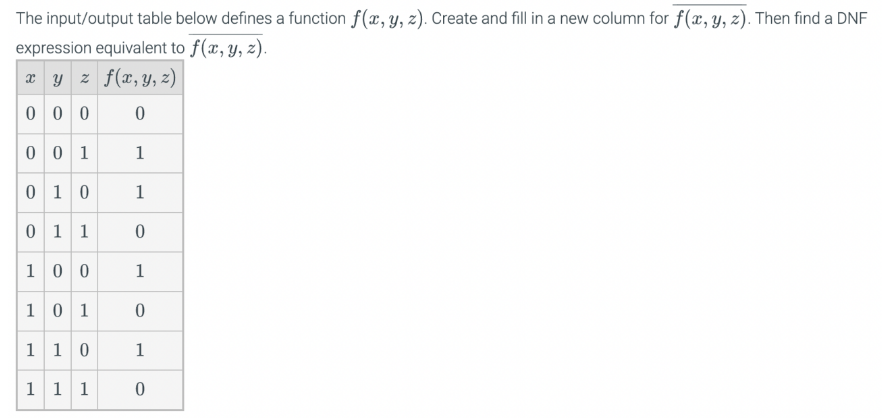
\includegraphics[scale=0.95]{question3.png}
    \item[] 
    $f(x,y,z) = \overline{xy}z + \overline{x}y\overline{z} + x\overline{yz} + xy\overline{z}$
    \item[]
    $\overline{f(x,y,z)} = xy\overline{z} + x\overline{y}z + \overline{x}yz + \overline{xy}z$

    \begin{displaymath}
        \begin{array}{|c|c|c|c|}
        % |c c|c| means that there are three columns in the table and
        % a vertical bar ’|’ will be printed on the left and right borders,
        % and between the second and the third columns.
        % The letter ’c’ means the value will be centered within the column,
        % letter ’l’, left-aligned, and ’r’, right-aligned.
        x & y & z & \overline{f(x,y,z)}\\ % Use & to separate the columns
        \hline % Put a horizontal line between the table header and the rest.
        0 & 0 & 0 & 0\\
        0 & 0 & 1 & 1\\
        0 & 1 & 0 & 0\\
        0 & 1 & 1 & 1\\
        1 & 0 & 0 & 0\\
        1 & 0 & 1 & 1\\
        1 & 1 & 0 & 1\\
        1 & 1 & 1 & 0\\
        \end{array}
    \end{displaymath}

    \item[4.] Describe a general method for taking a Boolean function defined by an input/output table and finding an
    equivalent CNF expression.
    \item[] First, look for all rows where the function evaluates to 0. The form for a CNF function is $\overline{row1}\cdot \overline{row2}\cdot ...$
    \item[] If the variable is 1, complement it, else do nothing. Multiply every row with each other. 
    \item[] The CNF function for the function in question 3 is $f(x,y,z) = (xyz)(x\overline{y}z)(\overline{x}yz)\overline{(xyz)}$. We use rows 1,3,5,8. We take all the values of x,y, and z, complementing when we see a 1 and multiply all rows together.
    \newpage
    \item[5.] For each expression below, give an equivalent expression that uses only the NAND operation. Then give an
    equivalent expression that uses only the NOR operation. (using boolean algebraic notations)
    \begin{enumerate}
        \item $\overline{x} + y$
        \item[] $\overline{x} + y = (x \uparrow \overline{y}) = x \uparrow (y \uparrow y)$
        \item[] $\overline{x} + y = \overline{x\overline{y}} = ((x \downarrow x) \downarrow y)\downarrow ((x \downarrow x)\downarrow y)$
        \item $\overline{(xy)}$
        \item[] $\overline{(xy)} = x \uparrow y$ This is what NAND is. 
        \item[] $\overline{(xy)} = ((x \downarrow x) \downarrow (y \downarrow y)) \downarrow ((x \downarrow x) \downarrow (y \downarrow y))$
    \end{enumerate}
    \item[6a.] Keeping the order of the elements fixed as 1, 2, 3, 4, 5, determine the (0, 1) relation matrix for each of
    the following equivalence relations.
    \item[] $R_1 = {(1, 1),(1, 2),(2, 1),(2, 2),(3, 3),(3, 4),(4, 3),(4, 4),(5, 5)}$
    \begin{equation}
        \begin{bmatrix}
            1 & 1 & 0 & 0 & 0\\
            1 & 1 & 0 & 0 & 0\\
            0 & 0 & 1 & 1 & 0\\
            0 & 0 & 1 & 1 & 0\\
            0 & 0 & 0 & 0 & 1
        \end{bmatrix}
    \end{equation}
    \item[] $R_2 = {(1, 1),(1, 2),(1, 3),(2, 1),(2, 2),(2, 3),(3, 1),(3, 2),(3, 3),(4, 4),(4, 5),(5, 4),(5, 5)}.$
    \begin{equation}
        \begin{bmatrix}
            1 & 1 & 1 & 0 & 0\\
            1 & 1 & 1 & 0 & 0\\
            1 & 1 & 1 & 0 & 0\\
            0 & 0 & 0 & 1 & 1\\
            0 & 0 & 0 & 1 & 1
        \end{bmatrix}
    \end{equation}
    \item[6b.]Do the results of part (a) lead to any generalization?
    \item[] Both of these graphs have 1's on the diagnols, which prove the fact that equivalence relations are reflexive. 
    \item[] Both of these graphs also supposed to be symmetric, since that is a defining property of equivalence relations. If we raise both matrix to any power, we still get that matrix. 
    \item[7.] Let $\left\lvert A \right\rvert  = 5$
    \begin{enumerate}
        \item How many directed graphs can one construct on A? 
        \item [] The number of directed graphs we can make is given by the equation $$2^{n(n-1)}$$
        \item [] If we plug in n=5, we get that the number of graphs we can create with 5 vertices is $2^20$.
        \item How many of the graphs in part (a) are actually undirected?
        \item [] We can use the equation $2^{\frac{n(n-1)}{2}}$ which gives us $2^{10}$ undirected graphs.
    \end{enumerate}
\end{enumerate}


\end{document}